\documentclass[a4paper, 11pt, final, garamond]{book}
\usepackage{cours-preambule}
\usepackage{pdfpages}

\raggedbottom

\makeatletter
\renewcommand{\@chapapp}{Travaux pratiques -- TP}
\makeatother

\let\SavedIndent\indent
\protected\def\indent{%
  \begingroup
    \parindent=\the\parindent
    \SavedIndent
  \endgroup
}
\setlength{\parindent}{0pt}

\begin{document}
\setcounter{chapter}{19}

\chapter{\'Etude des oscillations forc\'ees d'un oscillateur m\'ecanique amorti}
\section{Objectifs}

\begin{itemize}
    \item Utiliser un microcontrôleur Arduino afin de mettre en œuvre un
        accéléromètre.
    \item Tracer l'allure de la courbe de résonance en vitesse et en position.
    \item Vérifier les principales caractéristiques des oscillations mécaniques
        forcées.
    \item Déterminer le facteur de qualité du montage.
\end{itemize}

\section{S'approprier~: montage expérimental}

\begin{minipage}{0.60\linewidth}
    Une masse $m$, assimilée à un point matériel $M$, est suspendue entre deux
    ressorts dont l'un d'eux -- celui du haut -- est relié à un pot vibrant
    permettant d'induire un mouvement linéaire quasi sinusoïdal d'amplitude
    constante mais de fréquence réglable. Le déplacement du système vibrant dans
    l'air est à l'origine d'un amortissement fluide modélisé par une force du
    type~:
    \[
        \Ff = -\a\vf
    \]
    Un accéléromètre est attaché directement à la masse en translation verticale
    afin de suivre son déplacement au cours du temps. 
\end{minipage}
\hfill
\begin{minipage}{0.40\linewidth}
    \begin{center}
        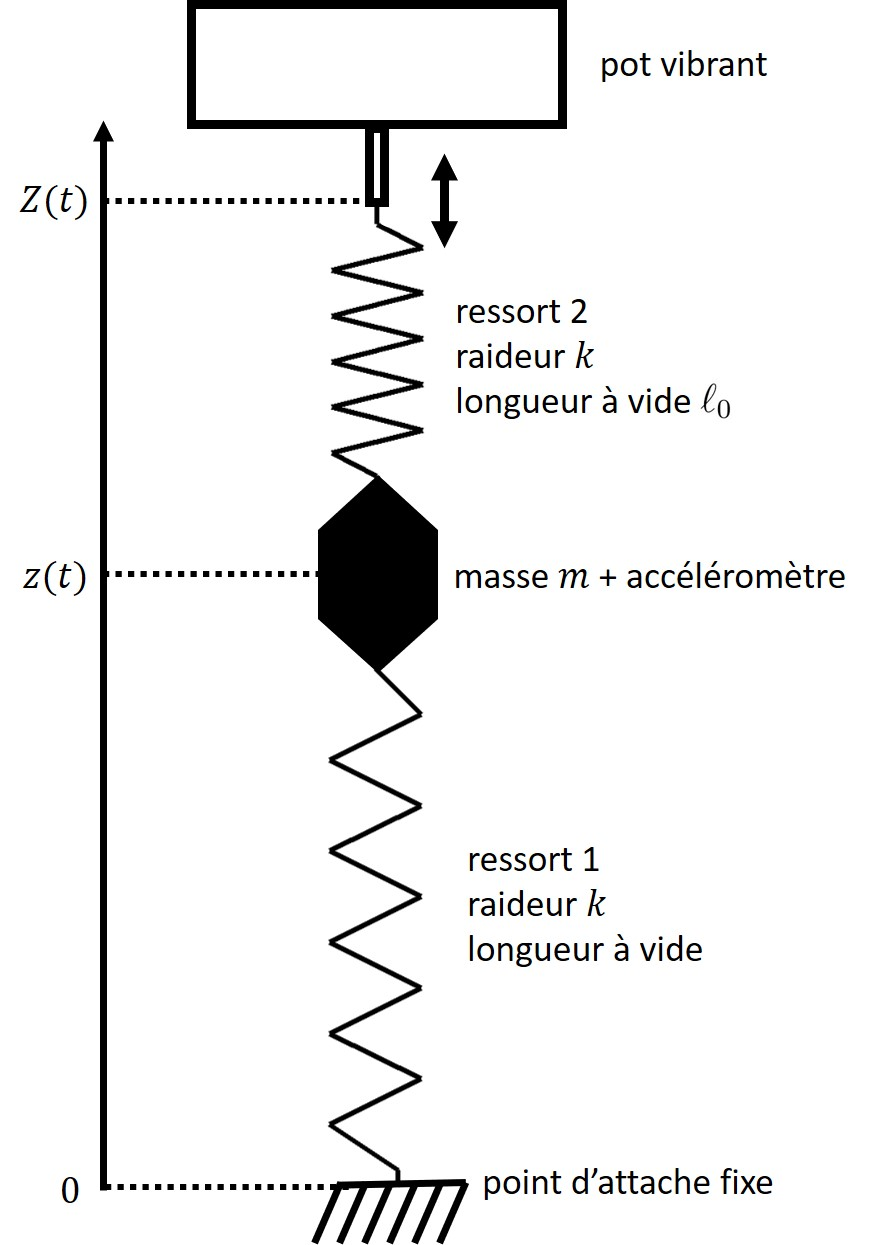
\includegraphics[height=7cm]{arduino_schema}
    \end{center}
\end{minipage}

\section{Analyser}

On repère la position de la masse $m$ grâce à son abscisse $z$ sur l'axe $(\Or
z)$ dont l'origine O est au point d'attache fixe du ressort $(1)$. Les deux
ressorts ont une longueur à vide $\ell_0$ et sont de raideur $k$.

\subsection{À excitation nulle}

À excitation nulle, on suppose que $z(t) = z_0$, une constante. 

\begin{enumerate}[label=\clenumi]
    \item Montrer que la longueur du ressort $(1)$ à l'équilibre est~: 
        \[
            \ell\ind{eq1} = z\ind{eq} = \frac{z_0}{2} - \frac{mg}{2k}
        \]
    \item On pose $u = z-z\ind{eq}$. Montrer que l'équation différentielle du
        mouvement de la masse $m$ peut se mettre sous la forme canonique~: 
        \[
            \ddot{u} + \frac{\w_0}{Q} \dot{u} + {\w_0}^2 u = 0
        \]
        Identifier $\w_0$ et $Q$, rappeler leur nom et leur unité.
    \item Quel est le ressort équivalent aux deux ressorts~?
\end{enumerate}

\subsection{En régime sinusoïdal forcé}

On se place en régime sinusoïdal forcé et on suppose que le point d'attache haut
du ressort (2) suit un mouvement sinusoïdal autour de sa position d'équilibre
$z_0$~: 
\[
    z(t) = z_0 + \alpha \cos(\w t)
\]

\begin{enumerate}[label=\clenumi, resume]
    \item Rappeler l'allure des courbes de résonance (amplitude en fonction de
        la fréquence) en position et en vitesse pour un tel système mécanique. À
        quel type de filtre cette fonction de transfert est-elle associée~?
    \item Quel lien existe-t-il entre l'amplitude du signal de position et du
        signal de vitesse~? 
    \item Quelle relation relie la bande passante et le facteur de qualité lors
        de la résonance en vitesse~?
\end{enumerate}

\subsection{Détection automatique de la fréquence et de l'amplitude}

Un signal réel est souvent bruité. Afin de détecter l'amplitude de
l'accélération, on réalise une transformée de Fourier numérique du signal. Un
pic dans le spectre apparaît autour de la fréquence d'excitation. En mesurant
l'amplitude de ce pic, on obtient (par le théorème de \textsc{Parseval})
l'amplitude du signal dans le domaine réel. Tout ce traitement est réalisé par
la fonction \texttt{freq\_finder} dans un script \texttt{Python}.

\section{Réaliser}

\subsection{Réglages}
\begin{enumerate}
    \item Brancher le GBF au \texttt{geneboost} par un câble coaxial. Le
        \texttt{geneboost} permet de délivrer le courant important demandé par
        le haut parleur mais ne modifie pas le signal de tension. 
    \item Relier le \texttt{geneboost} au haut parleur par une liaison bifilaire. 
    \item Régler le GBF sur une fréquence de $f = \SI{4}{Hz}$ et une tension
        crête à crête de $\SI{20}{Vpp}$.
    \item Attendre environ $\SI{30}{s}$ que le système atteigne le régime
        permanent avant de commencer toute mesure. Assurez vous que les
        oscillations soient bien verticales et qu'il n'y ait pas de rotation de
        la masselotte. Pour cela, régler la position du point d'attache bas en
        décalant ou tournant le contre-poids (point d'attache bas). Retenez vos
        fils à l'aide de la pince, ils ne doivent pas toucher la paillasse. 
    \item Ouvrir \texttt{Pyzo} et dans \texttt{Pyzo} ouvrir le script
        \texttt{Trace\_graphe\_accelerometre.py}.
    \item Faire une acquisition de l'accélération sur $\texttt{t\_acquisition} =
        \SI{5}{s}$. Une acquisition relativement longue est importante afin de
        traiter les données par la suite.
    \item Si le script s'interrompt, c'est une erreur dans la liaison série
        Arduino. Relancez simplement une nouvelle fois votre script. Ça devrait
        fonctionner correctement.
    \item Par ailleurs, entre deux acquisitions successives, appuyer sur
        \texttt{Ctrl + k} afin de réinitialiser le shell.
    \item En fin d'acquisition, déterminer l'amplitude du signal en accélération
        en calculant
        \[
            a = \frac{a\ind{max}-a\ind{min}}{2}
        \]
\end{enumerate}

\subsection{Acquisition et enregistrement}

\begin{enumerate}
    \item Ouvrir \texttt{Capytale} avec ce lien~:
        \url{https://capytale2.ac-paris.fr/web/c/3b87-1426775}
    \item Dans la cellule «~Données expérimentales~», créez trois listes avec~:
        \begin{enumerate}
            \item La tension d'alimentation (en \si{Vpp})
            \item La fréquence (en \si{Hz})
            \item L'amplitude de la réponse en accélération déterminée avec le
                script sur \texttt{Pyzo}.
        \end{enumerate}
    \item Faire une quinzaine d'acquisition entre $f\ind{min} = \SI{4}{Hz}$ et
        $f\ind{max} = \SI{15}{Hz}$. Vous resserrerez vos mesures autour de
        la résonance.
    \item Lorsque vous approchez de la résonance, l'amplitude $z(t)$ augmente
        significativement. Pour éviter d'endommager le système ou de saturer la
        mesure de l'accélération, on diminue l'amplitude de l'oscillation 
        en diminuant la tension crête à crête au niveau du GBF. C'est la raison
        pour laquelle vous devez \textbf{noter cette tension à chaque mesure}.  
\end{enumerate}

\section{Valider et conclure}
\subsection{Traitement des données}
Afin d'exploiter les enregistrements, effectuez, à partir des données
précédemment regroupées sur \texttt{Capytale}, les étapes suivantes \textbf{que
vous expliquerez sur votre copie} (d'où les $\fbox{1}$)~:

\begin{enumerate}[label=\sqenumi, start=7]
    \item Calculer la pulsation $\w$ de chaque enregistrement.
    \item L'amplitude de l'excitation en accélération est supposée
        proportionnelle à l'amplitude de la tension au GBF. Calculez alors
        l'amplitude en accélération que vous auriez si toutes les mesures
        avaient été effectuées pour une tension de $\SI{20}{Vpp}$. On notera
        cette grandeur $a_{20}$.
    \item Déterminer l'amplitude en vitesse puis en position à partir de
        $a_{20}$. Vous créerez pour cela deux nouvelles listes sur
        \texttt{Capytale}~: $v$ et $z$.
    \item Tracer la position et la vitesse de l'oscillateur en fonction de la
        pulsation $\w$.
    \item Ces deux courbes ont-elles l'allure attendue (vous vérifierez en
        particulier que les régimes asymptotiques soient approximativement
        cohérents)~? Les résonances se font-elles à la même pulsation~?
    \item Déterminer graphiquement la pulsation de résonance de l'oscillateur
        $\w_0$.
    \item Déterminer la bande passante de l'oscillateur, en déduire le facteur
        de qualité $Q$.
    \item Conclure. 
\end{enumerate}

\begin{center}
    \begin{framed}
        \Large Pensez à rendre votre projet sur \texttt{Capytale} pour que je le
        note~!
    \end{framed}
\end{center}

\subsection{Comparaison à la théorie} 
\begin{enumerate}
    \item À l'aide d'une balance, déterminer la masse $m$.
    \item Proposer un protocole (que vous réaliserez) afin de déterminer la
        raideur $k$ des ressorts utilisés dans l'expérience. 
    \item En déduire la valeur de la pulsation théorique $\w\ind{0théo}$.
        Comparer à la pulsation $\w_0$ précédemment obtenue. 
\end{enumerate}

\end{document}
